\section{Seguridad}
Un protocolo provee \textbf{cofidencialidad} si encripta los mensajes para prevenir que un atacante pueda leerlos. Si además oculta la cantidad de información o el destino del mensaje, entonces ofrece \textbf{Confidencialidad de tráfico}.

Un atacante que no puede leer el contenido del mensaje encriptado sigue siendo capaz de modificar los paquetes nterceptados a través de una red y generar contenido válido. Si el protocolo implementa técnicas para detectar si un paquete fue modificado en el camino, entonces se dice que ofrece \textbf{Integridad}.

Otra amenaza para el cliente es ser dirigido sin saberlo a un sitio web falso. Esto puede resultar de un \textbf{DNS Attack}, en el que se ingresa información falsa en un servidor DNS o en la caché del DNS de la computadora del cliente. Esto lleva a traducir una URL correcta en una dirección IP incorrecta. Un protocolo que garantiza que realmente está hablando con quien cree que está hablando se dice que proporciona \textbf{autenticación}. La autenticación implica integridad, ya que no tiene sentido decir que un mensaje proviene de un cierto participante si ya no es el mismo mensaje.

Si el atacante en vez de crear un sitio falso, logra modificar los archivos de uno existente, Ese es un problema de \textbf{control de acceso}: hacer cumplir las reglas sobre quién está autorizado a hacer qué. Los sitios web también han sido objeto de ataques de denegación de servicio (DoS), durante los cuales los clientes potenciales no pueden acceder al sitio web porque está siendo abrumado por solicitudes falsas.  Afecta el nivel de \textbf{disponibilidad}.

\subsection{Principios de cifrado}
El cifrado transforma un mensaje de tal manera que se vuelve ininteligible para cualquier parte que no tenga el secreto de cómo revertir la transformación. El remitente aplica una función de cifrado al mensaje de texto plano original y envía el resultado a través de la red. El receptor aplica una función de descifrado al mensaje que le llega para recuperar el mensaje original.

La transformación representada por una función de encriptado y su función de descifrado correspondiente se llama \textbf{cipher}.

Las funciones de cifrado y descifrado son de conocimiento público pero están parametrizadas por una clave secreta. Una razón para este principio es que si se depende de que el cifrado se mantenga en secreto, entonces hay que retirar el cifrado (no solo las claves) cuando sea vulnerado. Esto significa cambios potencialmente frecuentes de cifrado, lo cual es problemático, ya que toma mucho trabajo desarrollar uno nuevo. Además, una de las mejores formas de saber que un cifrado es seguro es usarlo durante mucho tiempo, si nadie lo rompe, probablemente lo sea.

Los mejores algoritmos de cifrado pueden evitar que el atacante deduzca la clave incluso cuando este conoce tanto el texto plano como el texto cifrado. Esto deja al atacante sin otra opción que probar todas las claves posibles usando fuerza bruta. La fuerza bruta puede ser computacionalmente ineficiente si se eligue un espacio de claves lo suficientemente grande y si las operaciones de cifrado y descifrado son lo suficientemente costosas. Una de las idifcultades de esta elección es que las velocidad de computo aumentan con el tiempo, por lo que lo que ahora puede ser computacionalmente imposible, en el futuro quizas sea posible.

\subsubsection{Cifrado en bloques}
La mayoría de los cifrados son \textbf{cifrados de bloque}: se definen para tomar como entrada un bloque de texto plano de un cierto tamaño fijo, típicamente de 64 a 128 bits. El uso de un cifrado de bloque para encriiptar cada bloque de forma independiente, conocido como \textbf{cifrado de libro electrónico (Electronic Cipher Book - ECB)}, tiene la debilidad de que un valor de bloque de texto plano dado siempre dará como resultado el mismo bloque de texto cifrado. Por lo tanto, los valores de bloque recurrentes en el texto plano son reconocibles como tales en el texto encriptado, lo que hace que sea mucho más fácil para un criptoanalista romper el cifrado.

Para evitar esto, los cifrados de bloque siempre se amplían para hacer que el texto resultate para un bloque varíe según el contexto. Las formas en que se puede ampliar un cifrado de bloque se llaman \textbf{modos de operación}. Un modo de operación común es el \textbf{Cipher Block Chaining (CBC)}, en el que cada bloque de texto plano se XORea con el texto cifrado del bloque anterior antes de ser encriptado. El resultado es que el texto cifrado de cada bloque depende en parte de los bloques anteriores. Dado que el primer bloque no tiene precedente, se lo xorea con un número random llamado \textbf{vector de inicialización} que se acuerda al principio de la comunicación para que el receptor pueda descifrarlo.

\subsubsection{Cifrados de clave secretas}
En un cifrado de clave secretas o clave simetrica, ambos participantes de la comunicación comparten la misma clave. Osea que el mensaje es encriptado usando una clave particular y luego es desencriptado usando la misma clave. El problema es que la clave debe ser compartida entre los participantes de la comunicación, lo que puede ser difícil de lograr. Además, si la clave se ve comprometida, entonces todos los mensajes encriptados con esa clave también se ven comprometidos.

El Instituto Nacional de Estándares y Tecnología (NIST) de los EE. UU. ha emitido estándares para una serie de cifrados de clave secreta. El \textbf{Estándar de cifrado de datos (Data Encryption Standard - DES)} fue el primero, y ha resistido la prueba del tiempo en el sentido de que no se ha descubierto ningún ataque criptanalítico mejor que la búsqueda de fuerza bruta. Sin embargo, las claves de DES son relativamente cortas (56 bits), lo que significa que un atacante con suficiente poder de cómputo puede probar todas las claves posibles en un tiempo razonable. Por lo tanto, DES ya no se considera seguro.

Se actualizó este estandar con el cifrado \textbf{3DES} que aplica tres claves DES (168 bits) para encriptar el mensaje de la siguiente manera:
\begin{enumerate}
  \item Usa la primer clave para encriptar el mensaje original.
  \item La segunda se usa para desencriptar el resultado del paso anterior. Osea se aplica la función de descifrado de DES para obtener un nuevo mensaje.
  \item La tercer clave se usa para encriptar el resultado del paso anterior. Osea se aplica la función de cifrado de DES para obtener el mensaje final.
\end{enumerate}

El desencriptado implica hacer la inversa de cada uno de esos pasos: Desencriptar con la tercer clave, encriptar con la segunda y desencriptar con la primera.

Actualmente, 3DES está siendo reemplazado por el estándar \textbf{Advanced Encryption Standard (AES)} emitido por NIST que soporta claves de 128, 192 y 256 bits.

\subsection{Cifrados de clave pública}
Una alternativa a los cifrados de clave secreta son los cifrados de clave pública. En lugar de una sola clave compartida por dos participantes, un cifrado de clave pública utiliza un par de claves relacionadas, una para el cifrado y otra diferente para el descifrado. El par de claves es "propiedad" de un solo participante. El propietario mantiene la clave de descifrado en secreto para que solo él pueda descifrar los mensajes; esa clave se llama \textbf{clave privada}. Además, hace pública la clave de cifrado para que cualquiera pueda cifrar mensajes que le estén destinados; esa clave se llama \textbf{clave pública}.

Para que un esquema de este tipo funcione, no debe ser posible deducir la clave privada a partir de la pública.

\begin{figure}[H]
	\centering
	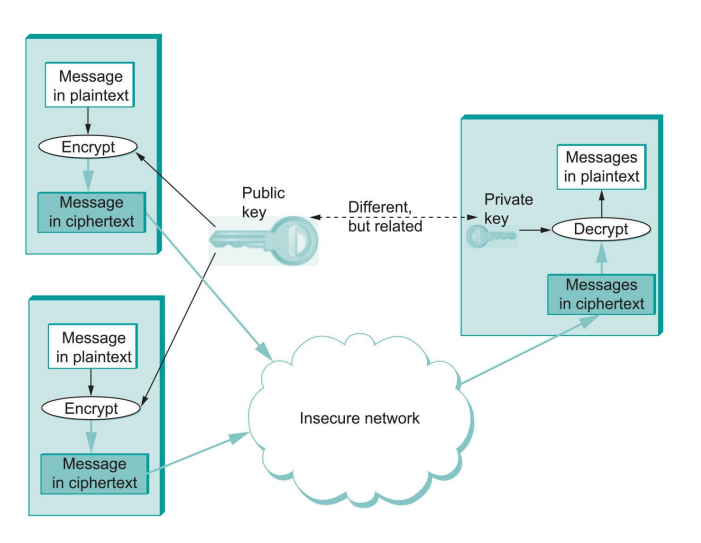
\includegraphics[width=0.5\textwidth
]{images/public-key-encryption.png}
	\caption[Encriptación con clave pública]{Encriptación con clave pública}
	\label{fig:public-key-encryption}
\end{figure}

Una clave para un cifrado de clave secreta proporciona un canal bidireccional entre dos participantes: cada participante tiene la misma clave (simétrica) que cualquiera puede usar para encriptar o desencriptar mensajes en cualquier dirección. Un par de claves pública / privada, en contraste, proporciona un canal unidireccional y de muchos a uno: desde todos los que tienen la clave pública hasta el único propietario de la clave privada.

Una propiedad adicional importante de los cifrados de clave pública es que la clave privada de "descifrado" se puede usar con el algoritmo de cifrado para cifrar mensajes de modo que solo se puedan descifrar usando la clave pública de "cifrado". Esta propiedad, si bien no nos ofrece confidencialidad, ya que cualquiera podría descifrar el mensaje, nos permite autenticar el mensaje. Si el mensaje se descifra correctamente, entonces el receptor pued estar seguro que el mensaje fue enviado por la persona que lo encriptó. Esto se llama \textbf{firma digital}.

El algoritmo de clave pública más conocido es el RSA (Rivest, Shamir, Adleman). Este algoritmo aprovecha el alto costo computacional de factorizar números grandes. El problema de encontrar una manera eficiente de factorizar números es uno en el que los matemáticos han trabajado sin éxito desde mucho antes de que apareciera RSA en 1978, y la resistencia posterior de RSA a la criptoanálisis ha fortalecido aún más la confianza en su seguridad. Desafortunadamente, RSA necesita claves relativamente grandes, al menos 1024 bits, para ser seguro. Las claves RSA son mas grandes que las claves para los cifrados de clave secreta porque es más rápido romper una clave privada RSA factorizando el número grande en el que se basa el par de claves que buscando exhaustivamente el espacio de claves.

En general, los cifrados de clave pública son usados principalmente para autenticar y distribuir claves secretas (simétricas) para su uso durante la comunicación entre dos entidades. Esto se debe a que los cifrados de clave pública son computacionalmente costosos en comparación con los cifrados de clave secreta.


\subsubsection{Autenticadores}
Un autenticador es un valor, que se incluye en un mensaje transmitido, que puede ser usado para verificar simultaneamente la autenticidad y la integridad de los datos de un mensaje.

Las sumas de verificación (checksums) y las comprobaciones de redundancia cíclica (CRC) son piezas de información agregadas a un mensaje para que el receptor detecte cuando el mensaje ha sido modificado inadvertidamente por errores de bits. Un concepto similar se aplica a los autenticadores, con el desafío adicional de que la corrupción del mensaje probablemente sea realizada deliberadamente por alguien que quiera que la corrupción pase desapercibida.

Para admitir la autenticación, un autenticador incluye alguna prueba de que quien creó el autenticador conoce un secreto que solo conoce el supuesto remitente del mensaje. 

\paragraph{Cryptographic checksum: }  Combina encriptación y una función hash criptográfica. Los algoritmos hash criptográficos se tratan como conocimiento público, como con los algoritmos de cifrado. Una función hash criptográfica (también conocida como suma de verificación criptográfica) es una función que produce suficiente información redundante sobre un mensaje para exponer cualquier manipulación. El resultado de esta función se llama \textbf{Message Digest} y se agrega al final del mensaje antes de encriptar. El receptor puede verificar la integridad del mensaje descifrando el mensaje y luego aplicando la función hash criptográfica al mensaje descifrado. Si el resultado coincide con el Message Digest recibido, entonces el mensaje no se ha modificado. 

Todos los message digests generados por la función son del mismo tamaño, idependientemente de la longitud del mensaje original. Dado que el espacio de mensajes posibles es más grande que el espacio de message digests, habrá mensajes distintos que tienen el mismo valor de message digest. Para que la función de hash sea segura en necesario que tenga la propiedad \textbf{one-way}: Debe ser computacionalmente imposible encontrar un mensaje que produzca el mismo message digest que el mensaje original. 

Una condición necesaria para que esto se cumpla es que el output de esta función debe estar distribuido uniformemente en el espacio de message digests. Si no lo está, entonces habrá regiones del espacio de message digests que son más probables que otras y, por lo tanto, más fáciles de encontrar.

Ha habido varios algoritmos hash criptográficos comunes a lo largo de los años, incluidos Message Digest 5 (MD5) y la familia Secure Hash Algorithm (SHA). Las debilidades de MD5 y las versiones anteriores de SHA han sido conocidas por algún tiempo, lo que llevó al NIST a recomendar el uso de SHA-3 en 2015.

\subsubsection{Firma Digital} Un digest encriptado con un algoritmo de clave pública pero usando la clave privada se llama firma digital porque proporciona no repudio como una firma escrita. El receptor de un mensaje con una firma digital puede demostrar a cualquier tercero que el remitente realmente envió ese mensaje, porque el tercero puede usar la clave pública del remitente para verificarlo por sí mismo.

\subsubsection{Message Authentication Code (MAC)} 
Se usa una clave secreta (conocida solo por el remitente y el receptor) para crear un código MAC que se concatena al mensaje de texto plano (antes de encriptar). Cuando el recptor recibe  el mensaje, calcul su propio MAC usando el texto del mensaje que le llegó y la clave secreta. Si el código MAC calculado coincide con el código MAC recibido, entonces el receptor puede estar seguro de que el mensaje no se ha modificado y que fue enviado por alguien que conoce la clave secreta. 

Una variación de este esquema es el \textbf{HMAC} en la que el mensaje se concatena la clave secreta y se pasa a una función de hash criptográfica. El resultado que devuelve está función es el codigo que se concatena al mensaje antes de ser enviado.

\subsection{Distribución de claves}
Para poder usar autenticadores o cifrado de clave secreta, los participantes deben saber qué claves usar.

\paragraph{Session Key:} Una clave secreta que se genera para su uso en una sola sesión de comunicación, es válida durante un pequeño intervalo de tiempo. Cada sesión tiene un clave diferente y esta es determinada por medio de algún protocolo de protocolo especial. 

\paragraph{Predistributed Keys:} Son claves que se distribuyen antes de que se necesiten. En general, son manejadas por un centro de administración de claves que permite a los usuarios establecer sesiones de comunicación segura entre ellos. En general, este tipo de claves solo se utiliza al comienzo de una comunicación para establecer una clave de sesión entre los participantes para luego pasar a usar esa clave de sesión para el resto de la comunicación.

Hay dos razones para que estas claves se usen de esta forma:
\begin{itemize}
  \item Limitar la cantidad de veces que se usa una clave resulta en menos tiempos para ataques que sean intensivos computacionalmente, menos texto cifrado que un atacante pueda interceptar y menos información expuesta si la clave se ve comprometida.
  \item Las claves públicas son superiores a las claves secretas en términos de autenticación y establecimiento de clave, pero es demasiado lento cifrar mensajes completos con ellas.
\end{itemize}

\subsubsection{Predistribución de claves públicas}
Los algoritmos para crear un par de claves publica/privadas son de público conocimiento y es facil de econtrar software que lo haga. 

Supongamos que Alice quiere usar cifrado asimétrico, entonces podría generar su propio par de claves y publicar la clave publica. El problema es como publicar la clave de tal maner que otros usuarios puedan estar seguros de que la clave publica realmente le pertenece a ella.

\subsubsection*{Public Key Infrastructure (PKI)}
Una PKI comienza con la capacidad de verificar identidades y vincularlas a claves fuera de banda. Por "fuera de banda", nos referimos a algo fuera de la red y de las computadoras que la componen, por ejemplo, si Alice y Bob son individuos que se conocen, entonces podrían reunirse en la misma habitación y Alice podría darle su clave pública a Bob directamente, tal vez en una tarjeta de presentación.

Establecer claves fuera de banda no parece que escalaría bien, pero es suficiente para arrancar una PKI. El conocimiento de Bob de que la clave de Alice es \(X\) puede ser ampliamente, difundido de forma escalable usando una combinación de firmas digitales y un concepto de confianza.

Una declaración firmada digitalmente de una vinculación de clave pública se llama \textbf{certificado de clave pública}, o simplemente certificado. Este certificado debe contener:
\begin{itemize}
  \item La identidad de la entidad que está siendo certificada.
  \item La clave pública de esa entidad.
  \item La identidad del que firma el certificado
  \item La firma digital
  \item Un identificador del algoritmo de firma digital que se usó para crear la firma.
\end{itemize}

\subsubsection*{Autoridades de certificación}
Si \(X\) certifica que una cierta clave pública pertenece a \(Y\), y luego \(Y\) certifica que otra clave pública pertenece a \(Z\), entonces existe una cadena de certificados de \(X\) a \(Z\), incluso si \(X\) y \(Z\) nunca se han conocido.

Una \textbf{autoridad de certificación} o \textbf{autoridad de certificados (CA)} es una entidad que se afirma que es confiable para verificar identidades y emitir certificados de clave pública.

Hay CA comerciales, CA gubernamentales e incluso CA gratuitas. Para usar una CA, se debe conocer su clave, la cual se puede aprender la clave de una CA si puede obtener una cadena de certificados que comienza con una CA cuya clave ya conoce. Luego puede creer cualquier certificado firmado por esa nueva CA. 

Una forma común de construir tales cadenas es organizarlas en una jerarquía estructurada en árbol. En la parte superior de la jerarquía se encuentra una CA raíz, que es una CA que se considera confiable sin necesidad de un certificado. La CA raíz emite certificados para otras CA, que a su vez emiten certificados para otras CA, y así sucesivamente. 

Hay algunos problemas importantes con la construcción de cadenas de confianza. Lo más importante es que, incluso si se está seguro de que se tiene la clave pública de la CA raíz, debemos asegurar que cada CA, desde la raíz hacia abajo, esté haciendo su trabajo correctamente. Si solo una CA en la cadena está dispuesta a emitir certificados a entidades sin verificar sus identidades, entonces lo que parece ser una cadena válida de certificados se vuelve insignificante.

Firefox e Internet Explorer vienen pre-equipados con certificados para un conjunto de CA; en efecto, el productor del navegador ha decidido que estas CA y sus claves pueden ser confiables. Un usuario también puede agregar CA a las que su navegador reconoce como confiables. Estos certificados son aceptados por Secure Socket Layer (SSL) / Transport Layer Security (TLS), el protocolo más utilizado para asegurar las transacciones web.

\subsubsection*{Web of trust}
Un modelo alternativo de confianza es la red \textbf{Pretty Good Privacy (PGP)}:  es un sistema de seguridad para correo electrónico, en el cual las direcciones de email son las identidades a las que se vinculan las claves y por las que se firman los certificados. En consonancia con las raíces de PGP como protección contra la intrusión del gobierno, no hay CA. En cambio, cada individuo decide en quién confía y cuánto confía en ellos; en este modelo, la confianza es una cuestión de grado. Un certificado puede incluir un nivel de confianza que indique cuán confiado está el firmante de la vinculación de claves reclamada en el certificado, por lo que un usuario determinado podrá decidir esperar varios certificados que atestigüen la misma vinculación de claves antes de estar dispuesto a confiar en ella.

En resumen, PGP reconoce que el problema de establecer la confianza es un asunto bastante personal y les da a los usuarios la materia prima para tomar sus propias decisiones en lugar de asumir que todos están dispuestos a confiar en una sola estructura jerárquica de CA.

\subsubsection*{Revocación de certificados}
En el caso de que un certificado haya sido vulnerado, las CA agrega este certificado a una \textbf{Lista de certificados revocados (Certificate Revocation List - CRL)} que firma digitalmente. Los usuarios pueden descargar la CRL y verificar si un certificado dado está en ella. Si lo está, entonces el certificado se ha revocado y no debe confiarse. Además, cada certificado tiene un tiempo de vida, después del cual se considera inválido y son eliminados de esta lista.

\subsubsection{Predistribución de claves secretas}
Existen entidades conocidas como \textbf{Key Distribution Centers (KDC)} que se encargan de distribuir claves secretas. Un KDC es un servidor que comparte una clave secreta con cada participante de la comunicación. Cuando Alice quiere comunicarse con Bob, se comunica con el KDC usando claves asimétricas indicandole sus intenciones. El KCD genera una clave secreta que le envia a Alice y a Bob. Luego Alice y Bob pueden comunicarse usando esa clave secreta.

\subsection{Protocolos
 de autenticación}
\paragraph{Reply Attack:} Un ataquente retransmite una copia de un mensaje que ya se envió. A pesar de que no es la primera encarnación del mensaje, el autenticador es válido y como no fue modificado puede ser correctamente descifrado. Sin embargo, el mensaje puede no ser válido en el contexto actual. Por ejemplo, si el mensaje es una solicitud de transferencia de fondos, entonces el atacante podría retransmitir la solicitud para que se ejecute dos veces. Necesitamos una solución que provea \textbf{Originalidad}.

Una veración de este ataque es el \textbf{supress-replay attack} en el que el atacante intercepta un mensaje y lo demora para que sea recibido en algún momento que no sea el apropiado. En este caso, aunque el mensaje es original, no es oportuno. Necesitamos una solución que provea \textbf{Timeliness}.

\subsubsection{Técnicas de Orginialidad y Timeliness}
Un enfoque es incluir una marca de tiempo en el mensaje. La marca de tiempo en sí debe ser a prueba de manipulaciones, por lo que debe estar cubierta por el autenticador. La principal desventaja de las marcas de tiempo es que requieren sincronización de relojes distribuidos. Dado que nuestro sistema dependería de la sincronización, la sincronización de relojes en sí misma debería defenderse contra las amenazas de seguridad, además de los desafíos habituales de la sincronización de relojes.

Otro enfoque es incluir, en el mensaje, un \textbf{nonce}, un número aleatorio que se usa solo una vez. Los participantes pueden detectar ataques de repetición verificando si un nonce se ha usado previamente. Desafortunadamente, esto requiere que se mantenga un log de los nonces ya usados, lo que puede ser difícil de escalar.

\begin{figure}[H]
	\centering
	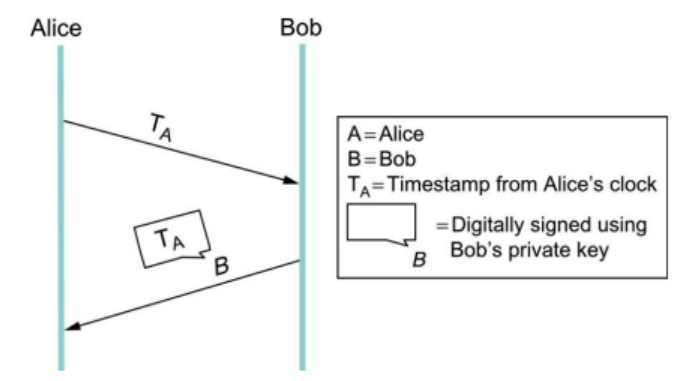
\includegraphics[width=0.5\textwidth
]{images/response-challenge-protocol.png}
	\caption[Protocolo response-challenge]{Protocolo response-challenge basado en timestamps}
	\label{fig:response-challenge-protocol}
\end{figure}

\subsubsection*{Protocolos de autenticación de clave asimétrica}
\begin{figure}[H]
	\centering
	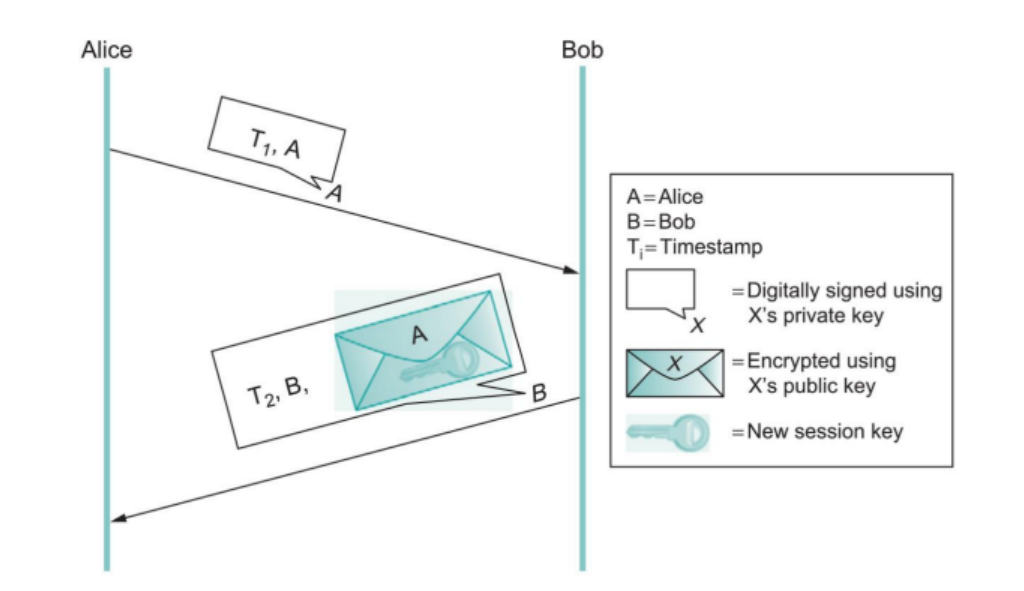
\includegraphics[width=0.5\textwidth
]{images/public-key-authentication.png}
	\caption[Protocolo de autenticación con clave asimétricas]{Protocolo de autenticación con clave asimétricas con sincronización de clocks}
	\label{fig:public-key-authentication}
\end{figure}

Alice envía a Bob un mensaje con un timestamp y su identidad en texto plano más su firma digital. Bob usa la firma digital para autenticar el mensaje y el timestamp para verificar su frescura. Bob envía un mensaje de vuelta con una timestamp y su identidad en texto plano, así como una nueva clave de sesión encriptada (para confidencialidad) usando la clave pública de Alice, todo firmado digitalmente. Alice puede verificar la autenticidad y la frescura del mensaje, por lo que sabe que puede confiar en la nueva clave de sesión. Para lidiar con la sincronización imperfecta del reloj, las marcas de tiempo podrían aumentarse con nonces.

\begin{figure}[H]
	\centering
	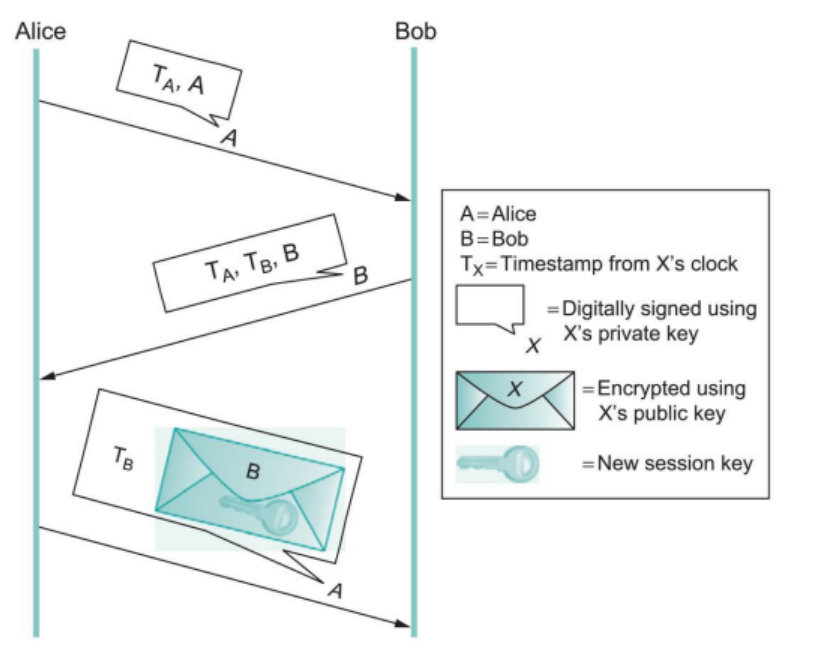
\includegraphics[width=0.5\textwidth
]{images/public-key-authentication-2.png}
	\caption[Protocolo de autenticación con clave asimétricas]{Protocolo de autenticación con clave asimétricas sin sincronización de clocks}
	\label{fig:public-key-authentication-2}
\end{figure}
En este protocolo, Alice nuevamente envía a Bob un mensaje firmado digitalmente con una marca de tiempo y su identidad. Debido a que sus relojes no están sincronizados, Bob no puede estar seguro de que el mensaje sea nuevo. Bob envía un mensaje firmado digitalmente con la marca de tiempo original de Alice, su propia marca de tiempo y su identidad. Alice puede verificar la frescura de la respuesta de Bob comparando su tiempo actual con la marca de tiempo que se originó con ella. Luego le envía a Bob un mensaje firmado digitalmente con su marca de tiempo original y una nueva clave de sesión encriptada usando la clave pública de Bob. Bob puede verificar la frescura del mensaje porque la marca de tiempo provino de su reloj, por lo que sabe que puede confiar en la nueva clave de sesión. Las marcas de tiempo esencialmente sirven como nonces convenientes, e incluso este protocolo podría usar nonces en su lugar.

\subsubsection*{Protocolos de autenticación de clave simétrica}
\begin{figure}[H]
	\centering
	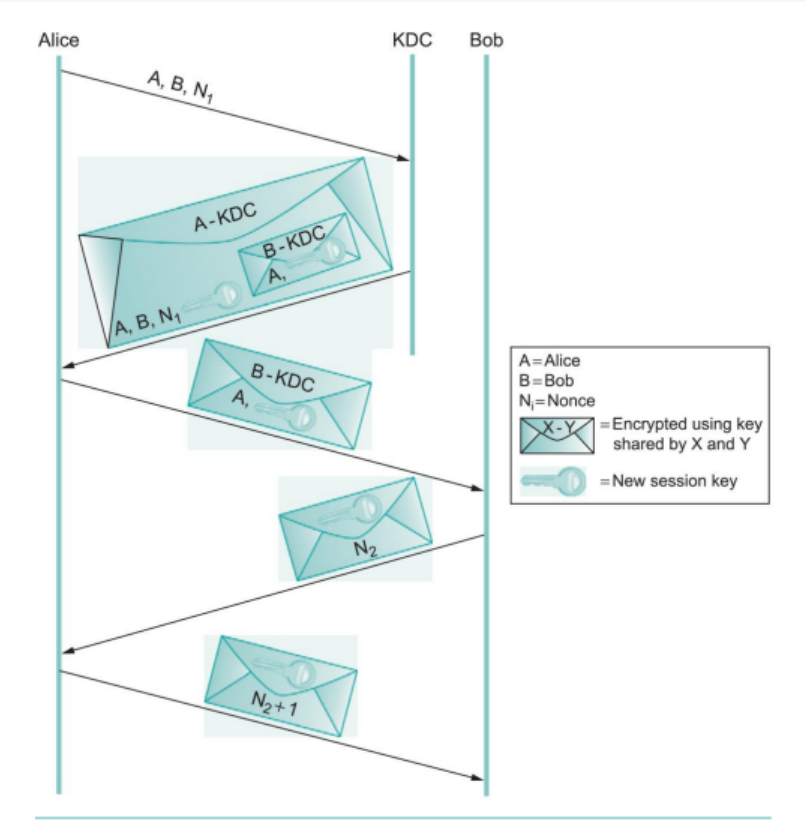
\includegraphics[width=0.5\textwidth]{images/kcd-autenthication.png}
	\caption[Protocolo de autenticación con KDC]{Protocolo de autenticación con KDC}
	\label{fig:kcd-authentication}
\end{figure}
El nonce en los primeros dos mensajes es para asegurarle a Alice que la respuesta del KDC es fresca. Los segundos y terceros mensajes incluyen la nueva clave de sesión y la identificación de Alice, encriptados juntos usando la clave maestra de Bob. Es una especie de versión de clave secreta de un certificado de clave pública; es, en efecto, una declaración firmada por el KDC (porque el KDC es la única entidad además de Bob que conoce la clave maestra de Bob) que la clave de sesión adjunta es propiedad de Alice y Bob.

Notar que el KDC no autentica realmente el mensaje inicial de Alice y no se comunica con Bob en absoluto. En cambio, utiliza su conocimiento de las claves públicas de Alice y Bob para construir una respuesta que sería inútil para cualquier persona que no sea Alice (porque solo Alice puede descifrarla) y que contiene los ingredientes necesarios para que Alice y Bob realicen el resto del protocolo de autenticación ellos mismos.
